\documentclass[conference]{IEEEtran}
\usepackage{graphicx}
\usepackage{tikz}
\usepackage{graphicx}

\usepackage[colorlinks = true, citecolor = blue]{hyperref}

% math lib
\usepackage{amsmath}
\usepackage{mathrsfs}

% operators
\DeclareMathOperator*{\argmax}{arg\,max}
\DeclareMathOperator*{\argmin}{arg\,min}
\newcommand\ceiling[1]{\left\lceil #1 \right\rceil}

% empty set
\usepackage{amssymb}
\let\emptyset=\varnothing

% algorithms
\usepackage{algorithm}
\usepackage{algorithmic}
\renewcommand{\algorithmicrequire}{\textbf{Input:}}
\renewcommand{\algorithmicensure}{\textbf{Output:}}

\begin{document}
% --------------------------------------------
% --------------Change HERE! -----------------
% --------------------------------------------
\def\authorone{Prabhat Edupuganti}
\def\authortwo{Rajiv Karthik Reddy Kodimala}
\def\groupid{9}
% --------------------------------------------
\title{CS258 Final Report: The RSA Problem}
\author{
    \IEEEauthorblockN{\authorone\ and \authortwo}
    \IEEEauthorblockA{
        Group \groupid
    }    
}

\maketitle
\IEEEpeerreviewmaketitle


\section{\textbf{Methods: RL-based Routing}}
\subsection{\textbf{RL Algorithms}}
% List RL algorithms and give a brief explanation of each

We have used two RL algorithms, Deep Q-Network (DQN)  Proximal and Policy Optimization (PPO) to train the model.

\subsubsection{\textbf{Deep Q-Network (DQN)}}
Deep Q-Network (DQN) \cite{Mnih2015} is a value-based method in reinforcement learning that combines Q-learning with deep neural networks to approximate the Q-value function, which estimates the expected future rewards of state-action pairs. It is based on Q-learning, a reinforcement learning algorithm that seeks to learn the optimal action-value function, Q(s, a), indicating the expected reward for taking action a in state s and following the optimal policy thereafter. DQN uses a neural network to handle high-dimensional state spaces and employs an experience replay buffer to store transitions and sample mini-batches during training, which helps break the correlation between consecutive transitions and improves stability. %Additionally, DQN uses a target network that is periodically updated to match the weights of the main Q-network, further stabilizing training by reducing correlations between target and predicted Q-values. This method is capable of handling complex state spaces and benefits from stabilized learning processes, making it more robust than vanilla Q-learning.DQN has been widely studied and improved upon, leading to various extensions such as Double DQN, Dueling DQN, and Prioritized Experience Replay.
% DQN is a value-based method in reinforcement learning.
% It combines Q-learning with deep neural networks to approximate the Q-value function, which estimates the expected future rewards of state-action pairs.
% Key Features:

% Q-Learning: DQN is based on Q-learning, a reinforcement learning algorithm that seeks to learn the optimal action-value function, Q(s, a), which tells the expected reward for taking action a in state s and following the optimal policy thereafter.
% Neural Networks: DQN uses a neural network to approximate the Q-values for each state-action pair, enabling it to handle high-dimensional state spaces that traditional Q-learning cannot.
% Experience Replay: DQN uses an experience replay buffer to store transitions (state, action, reward, next state) and samples mini-batches from this buffer during training. This helps break the correlation between consecutive transitions and improves training stability.
% Target Network: DQN employs a target network that is periodically updated to match the weights of the main Q-network. This helps stabilize training by reducing the correlations between the target and predicted Q-values.
% Advantages:

% High-Dimensional States: DQN can handle complex state spaces, such as those represented by images, thanks to its use of deep neural networks.
% Stabilized Learning: The use of experience replay and a target network helps stabilize the learning process, making it more robust than vanilla Q-learning.
% Well-Established: DQN is one of the first successful applications of deep learning in reinforcement learning and has been widely studied and improved upon, leading to various extensions like Double DQN, Dueling DQN, and Prioritized Experience Replay.

\subsubsection{\textbf{Proximal Policy Optimization (PPO)}}
Proximal Policy Optimization (PPO) \cite{schulman2017proximal} is a policy gradient method in reinforcement learning designed to update policies within a small, manageable range, thus preventing large, potentially destructive updates. It directly optimizes the policy using a clipped objective function to ensure the new policy does not deviate excessively from the old policy, stabilizing training. PPO employs a surrogate objective function to approximate the expected reward, making the optimization process more efficient, and performs multiple epochs of gradient descent on sampled data to improve the policy within the clipped range. %This method offers stable training by limiting policy update extents, greater sample efficiency by allowing multiple updates on the same data batch, and simplicity in implementation and tuning compared to more complex algorithms like Trust Region Policy Optimization (TRPO).


% PPO is a type of policy gradient method in reinforcement learning.
% It is designed to update policies in a way that keeps changes within a small, manageable range, thus preventing large, potentially destructive updates.
% Key Features:

% Policy-Based: PPO directly optimizes the policy that the agent uses to decide actions.
% Clipped Objective: PPO uses a clipped objective function to ensure that the new policy does not deviate too much from the old policy, which helps stabilize training.
% Surrogate Objective: PPO uses a surrogate objective function to approximate the expected reward, making the optimization process more efficient.
% Multiple Updates: PPO performs multiple epochs of gradient descent on the sampled data to improve the policy within the clipped range.
% Advantages:

% Stable Training: By limiting the extent of policy updates, PPO avoids the instability seen in other policy gradient methods.
% Sample Efficiency: PPO is more sample efficient than traditional policy gradient methods because it allows multiple updates on the same batch of data.
% Simplicity: PPO is relatively easy to implement and tune compared to more complex algorithms like Trust Region Policy Optimization (TRPO).



 Both PPO and DQN are powerful algorithms with distinct approaches to solving reinforcement learning problems, and their selection depends on the specific requirements and constraints of the problem at hand.

% Summary
% PPO: A policy gradient method that focuses on stabilizing updates to the policy by clipping the objective function. It allows multiple updates on the same batch of data and is known for its stability and simplicity.
% DQN: A value-based method that approximates the Q-value function using deep neural networks. It stabilizes training with techniques like experience replay and target networks, enabling it to handle high-dimensional state spaces effectively.
% Both PPO and DQN are powerful algorithms with distinct approaches to solving reinforcement learning problems, and their selection depends on the specific requirements and constraints of the problem at hand.

















\subsection{\textbf{State Space}}
% Explain state/action/reward
% Make sure you provide enough information to reconstruct results
% Check https://gymnasium.farama.org/environments/box2d/lunar_lander/ for some examples

The state space in our NetworkEnv class is defined as a 3D NumPy array with dimensions \begin{verbatim}
(num_nodes, num_edges, link_capacity)
\end{verbatim}

\noindent The state space is initialized as a zero-filled NumPy array, indicating that no connections are active at the start. Each entry in the 3D state array represents the holding time for a particular color (or slot) on a specific edge for a specific node.

\begin{verbatim} self.state[node, edge, color]
\end{verbatim}
The value at the position represents the remaining holding time for a connection using the color slot on the edge for the node.
\begin{verbatim} 
Example: self.state[0, 1, 2] = 15
\end{verbatim}
This means that for node 0, on edge 1, using color slot 2, there is a connection with a holding time of 15 units.

\subsection{\textbf{Action Space}}


The action space is a flattened representation of all possible combinations of edges and color slots (link capacities). The action space is flattened such that each action corresponds to a unique combination of an edge and a color slot. The total number of actions is the product of the number of edges and the number of color slots.

\begin{verbatim} Total Actions: num_edges * link_capacity
\end{verbatim}
For example, if there are 15 edges and 10 color slots, the action space size will be 15 * 10 = 150.

\noindent\textit{Flattening:} To flatten the action space, the action index is calculated as

\begin{verbatim}
action_index = edge_index * link_capacity 
                + color_slot
\end{verbatim}

\noindent\textit{Unflattening:} To retrieve the original edge and color slot from a given action index

\begin{verbatim}
edge_index = action // link_capacity
color_slot = action % link _capacity
\end{verbatim}


\subsection{\textbf{Reward Function}}

\noindent\textit{1. Default Reward for Invalid Actions:}
At the start of the step function, the default reward is set to -1. This is the penalty for taking an invalid action (e.g., choosing an edge that is not connected or selecting an already occupied slot without maintaining continuity).

\noindent\textit{2. Valid Action Reward:}
If the action is valid, the agent can receive a positive reward. The criteria for a valid action include:

The edge must be connected.
The color slot on the edge must be available (i.e., the holding time must be zero).
The selected color slot must either be the first action or continue from the previous edge with the same color slot for continuity.
For above action reward with value 5 is assigned.

\noindent\textit{3. High Reward for Reaching the Target Node:}
If the action leads to the target node, a high reward with value 20 is assigned. This is to incentivize the agent to find paths that reach the target node.

\noindent\textit{4. Network Utilization Reward:}
The reward also includes a component based on the network-wide utilization. This encourages the agent to maximize the utilization of the network's resources.

\textit{Total Utilization:} Tracks the number of used slots across all edges and color slots.
\textit{Average Utilization:} The mean utilization of all edges.
\textit{Network-Wide Utilization:} The overall mean utilization of the network.
The utilization reward is added to the base reward.

\begin{tiny}
\begin{verbatim}
# Calculate average utilization U(e) for each edge
average_utilization = np.sum(self.total_utilization, axis=1) / self.link_capacity

\# Calculate network-wide utilization U
network_utilization = np.mean(average_utilization)

reward += network_utilization  # Include network utilization in the reward

\end{verbatim}
\end{tiny}

    
        

\section{\textbf{Method: Spectrum Allocation}}\hfill
% Explain your heuristic
% If you have multiple, you can make subsections 

% If you borrow some ideas from papers, cite them with bibtex (e.g. \cite{8509143})

\subsubsection{\textbf{Detailed Explanation of State Management and Action Handling in NetworkEnv for RL Algorithms}}\hfill\\

\noindent\textbf{State Updates and Action Handling}

 \textit{State Updates in Step Function:} The state is updated in the step function when the agent takes an action. Actions involve assigning a holding time to a specific edge and color slot.

\textit{Action Unflattening:} The action is unflattened into an edge index and a color slot. If the edge and color slot are valid and not currently in use, the holding time for that slot is set.\\

\noindent\textbf{Holding Time Decrement and Partial Reset}

\textit{Passage of Time Simulation:} After each episode (request), the holding times in the state space are decremented to simulate the passage of time.

\textit{Partial Reset at Episode Start:} The state is partially reset at the start of each episode. If the environment runs out of pre-generated requests, it fully resets.\\

\noindent\textbf{Full Reset vs. Partial Reset}

\textit{Full Reset:} When all requests are processed, both the state and the utilization are reset to zero.

\textit{Partial Reset:} Only the holding times are decremented, and utilization is updated accordingly.\\

\noindent\textbf{Decrementing Holding Times}

\textit{Decrement Process:} For each active connection (i.e., each slot with a non-zero holding time), the holding time is decremented by 1. This simulates the passing of one time unit, indicating that the connection has been active for one more unit of time.\\

\noindent\textbf{Updating Utilization Metrics}

\textit{Utilization Update:} After decrementing the holding times, the utilization metrics are updated to reflect the current state of the network. If a holding time reaches zero, it means that the slot is now free, and this should be reflected in the utilization metrics.\\

\noindent\textbf{Validating and Applying Actions}\\
\textit{Action Validation:} When the agent takes an action, the environment unflattens the action to get the edge and color slot, then checks if the action is valid and updates the state accordingly.

\textit{Action Validity Check:} The environment checks the validity of the action before updating the state:
The edge must exist in the graph.
The selected color slot on the edge must be available (i.e., not currently in use).
The action should either be the first action taken or continue from the previous edge with the same color slot for continuity.
\\

\subsubsection{\textbf{Explanation of Simple Heuristic for Spectrum Allocation:}}

In our optical network, we employ the NetworkX shortest\_path() function to determine the optimal route between the source and target nodes for each connection request. Once the shortest path is identified, we apply the First-Fit heuristic to allocate spectrum slots along this path. The algorithm traverses the spectrum slots in a fixed order, selecting the first set of contiguous and continuous slots that meet the connection's requirements. 

\section{\textbf{Results}}

\subsection{\textbf{Learning Curve}}
% Insert figures
% Explain the results


\begin{figure}[H]
    \centering
    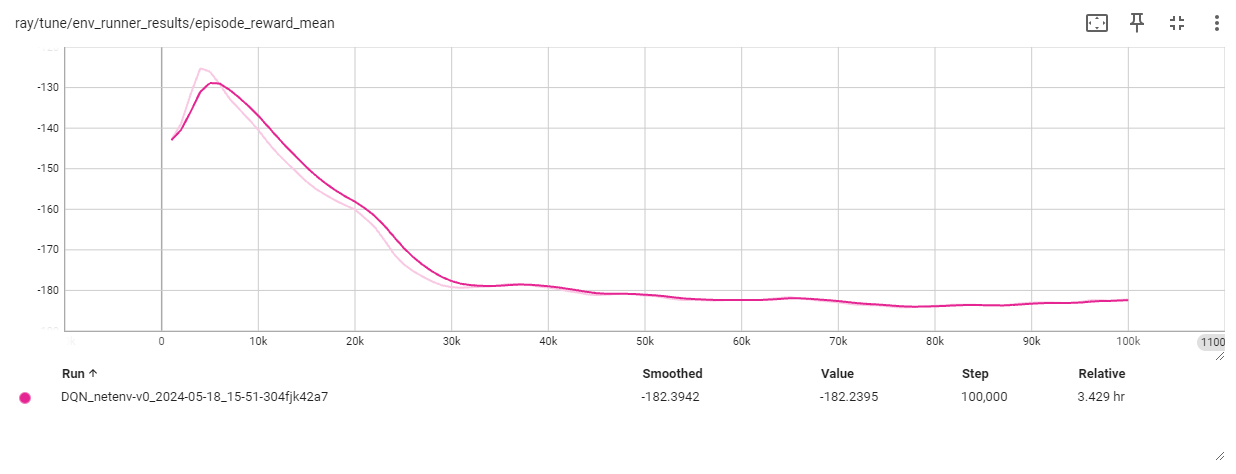
\includegraphics[width=0.5\linewidth]{dqn_fixed_reward.png}
    \caption{Case 1 : DQN\ episode\_reward\_mean}
    \label{fig:enter-label}
\end{figure}

\begin{figure}[H]
    \centering
    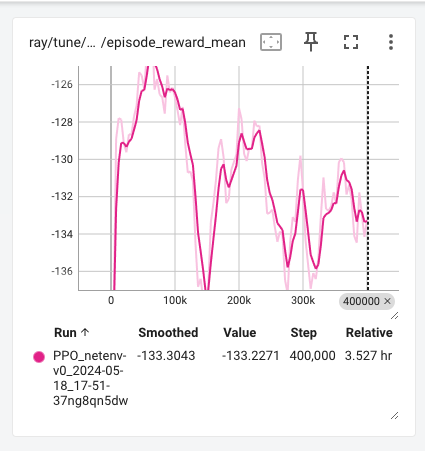
\includegraphics[width=0.5\linewidth]{ppo_fixed_reward.png}
    \caption{Case 1 : PPO\ episode\_reward\_mean}
    \label{fig:enter-label}
\end{figure}

\begin{figure}[H]
    \centering
    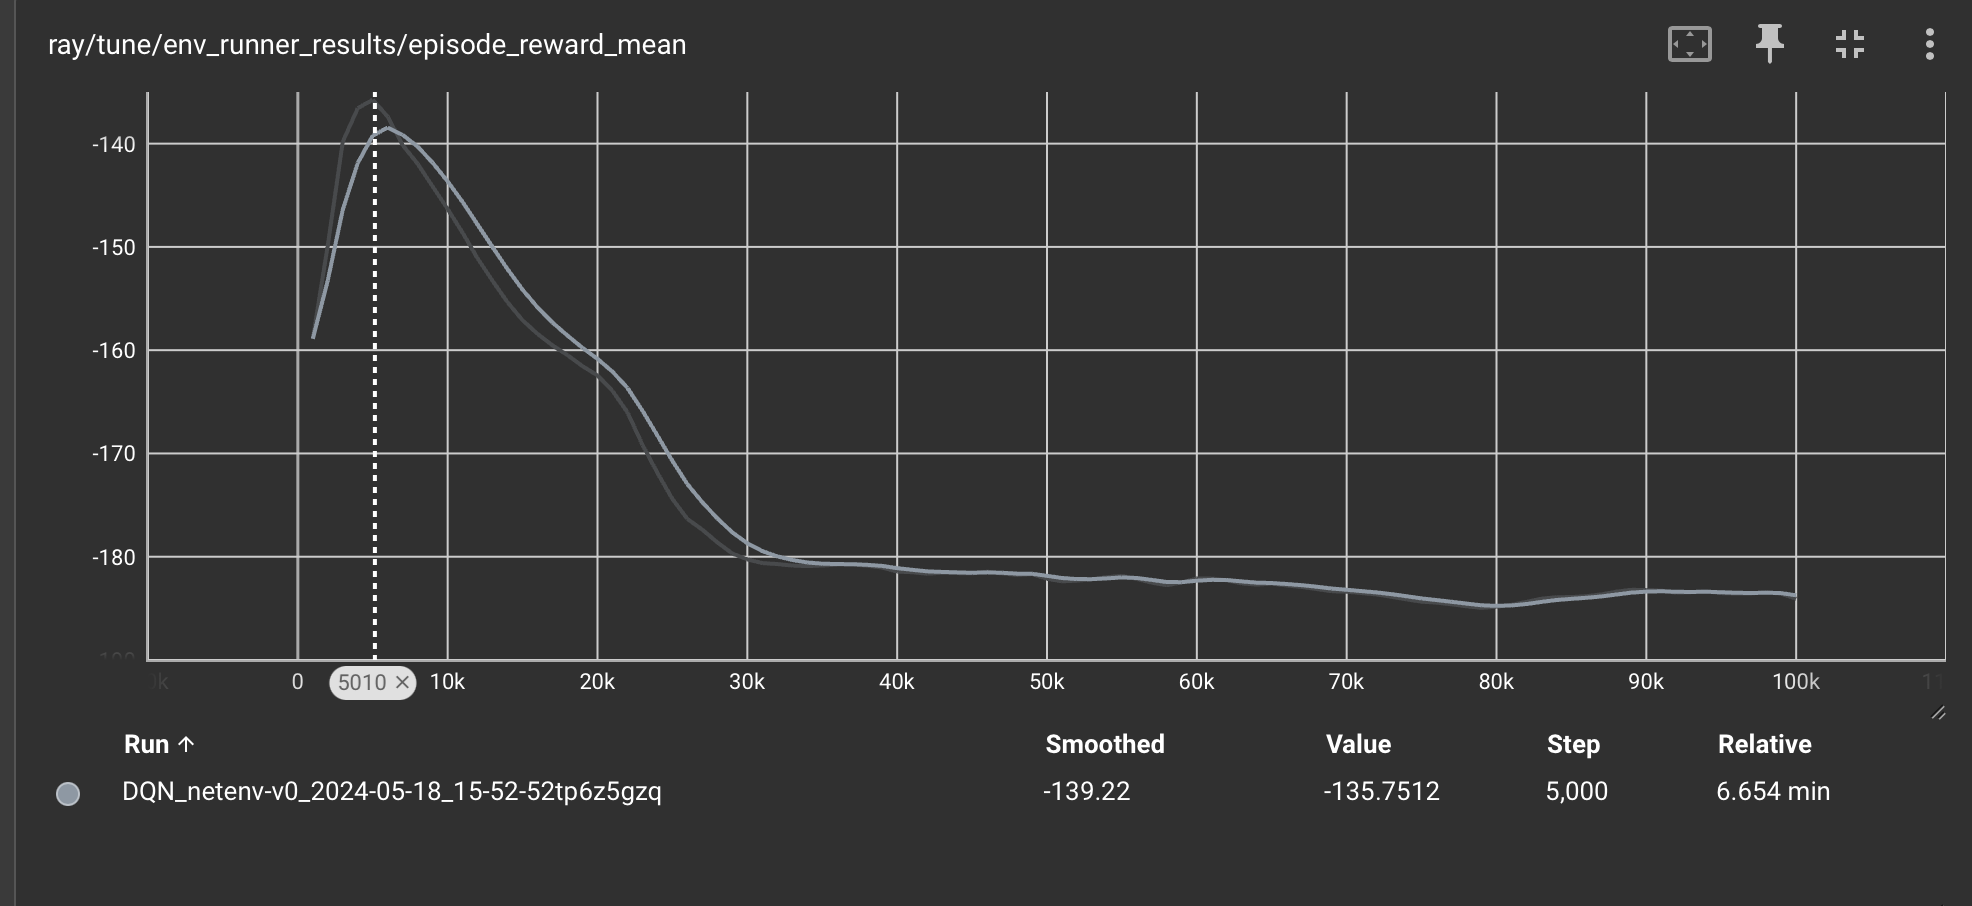
\includegraphics[width=0.5\linewidth]{dqn_random_reward.png}
    \caption{Case 2 : DQN\ episode\_reward\_mean}
    \label{fig:enter-label}
\end{figure}

\begin{figure}[H]
    \centering
    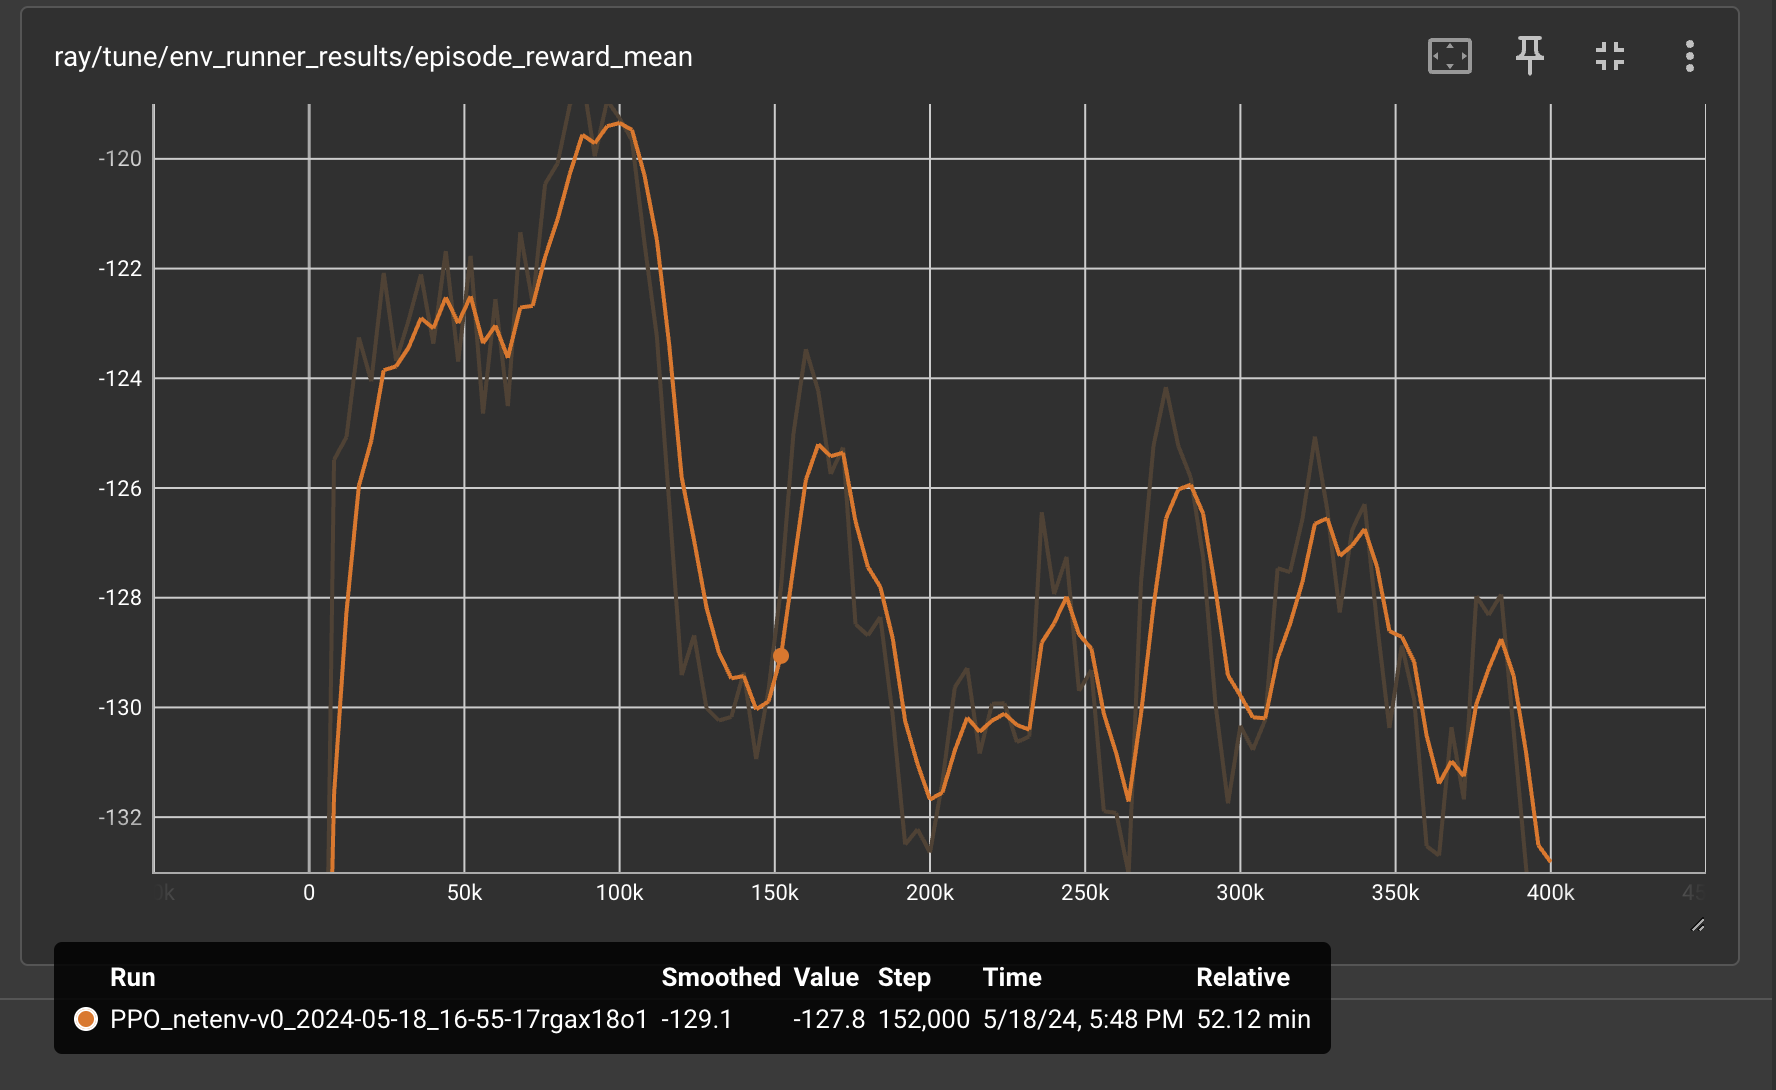
\includegraphics[width=0.5\linewidth]{ppo_random_reward.png}
    \caption{Case 2 : PPO\ episode\_reward\_mean}
    \label{fig:enter-label}
\end{figure}





\subsection{\textbf{Utilization (The Objective)}}
\begin{figure}[H]
    \centering
    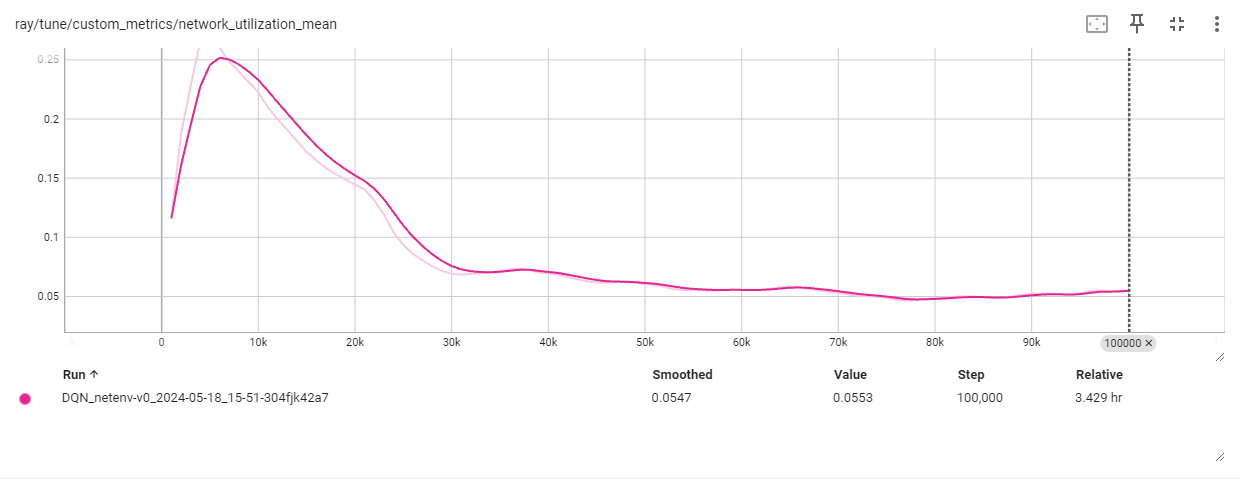
\includegraphics[width=0.5\linewidth]{dqn_fixed_ut.png}
    \caption{Case 1 : DQN\ network\_utilization\_mean}
    \label{fig:enter-label}
\end{figure}

\begin{figure}[H]
    \centering
    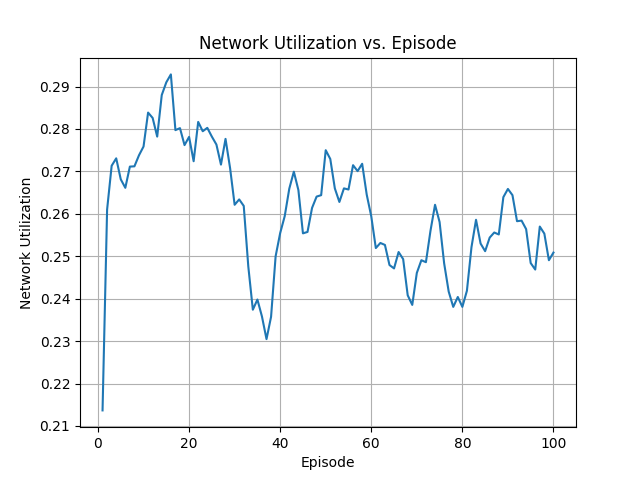
\includegraphics[width=0.5\linewidth]{ppo_fixed_uti.png}
    \caption{Case 1 : PPO\ network\_utilization\_mean}
    \label{fig:enter-label}
\end{figure}

\begin{figure}[H]
    \centering
    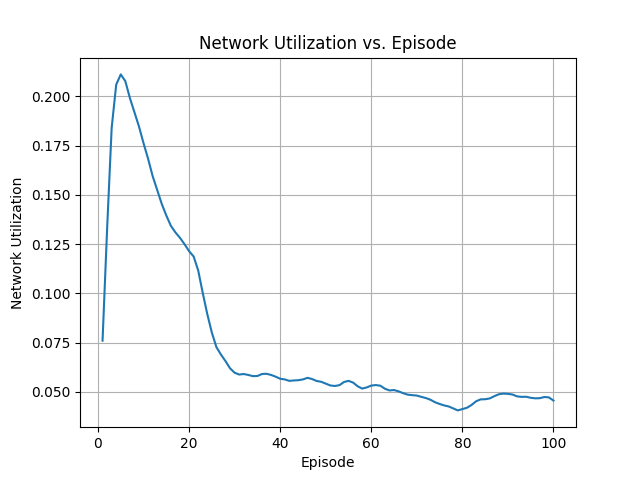
\includegraphics[width=0.5\linewidth]{dqn_random_uti.png}
    \caption{Case 2 : DQN\ network\_utilization\_mean}
    \label{fig:enter-label}
\end{figure}

\begin{figure}[H]
    \centering
    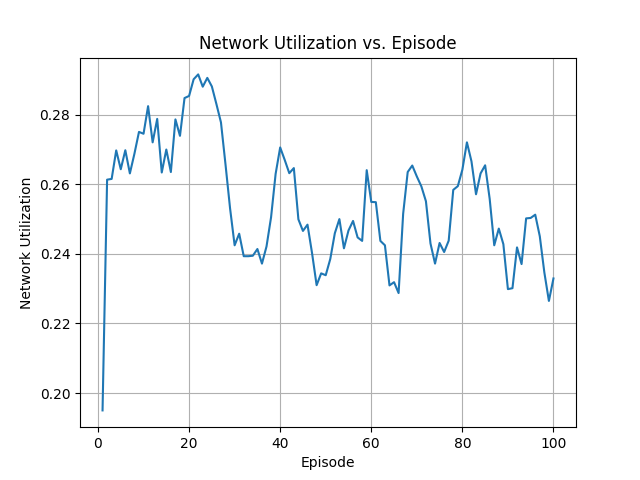
\includegraphics[width=0.5\linewidth]{ppo_random_uti.png}
    \caption{Case 2 : PPO\ network\_utilization\_mean}
    \label{fig:enter-label}
\end{figure}

\begin{figure}[H]
    \centering
    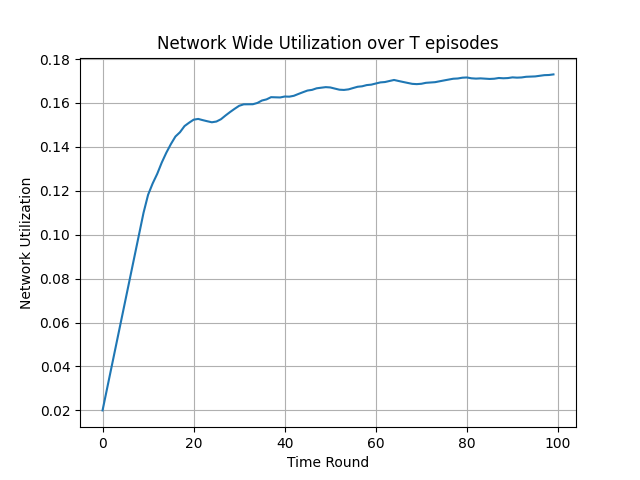
\includegraphics[width=0.5\linewidth]{FirstFit_ut1.png}
    \caption{Case 1 : First Fit network utilization}
    \label{fig:enter-label}
\end{figure}

\begin{figure}[H]
    \centering
    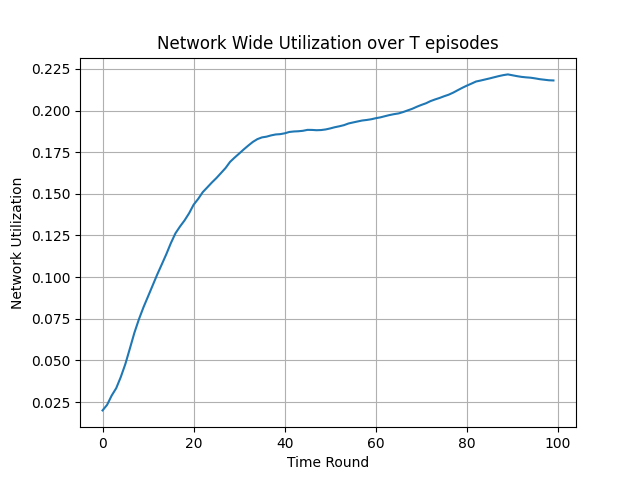
\includegraphics[width=0.5\linewidth]{FirstFit_ut2.png}
    \caption{Case 2 : First Fit network utilization}
    \label{fig:enter-label}
\end{figure}

The training time for 100 episodes in all the mentioned settings was close to 3 hours each.

Example: Run started at 1716072678.2126956 and ended at 1716085146.6709657. Elapsed time: 12468.458270072937 seconds

\subsection{\textbf{Comparison}}
We compared the values of the objective function obtained by two Reinforcement Learning (RL) methods, Deep Q-Network (DQN) and Proximal Policy Optimization (PPO), with those obtained by simple heuristics. Our results show that both RL algorithms outperform the heuristics in optimizing the objective function. Specifically, in the fixed source and target setting, DQN and PPO achieved peak network-wide utilization of 0.25 and 0.3, respectively, while the simple heuristic peaked at 0.18. Similarly, in the random source and target setting, DQN and PPO achieved peak utilization of 0.21 and 0.3, respectively, compared to 0.225 for the simple heuristic. These results demonstrate the effectiveness of RL methods in optimizing the objective function, and we discuss potential methods to further improve these results in the next section.

\subsection{\textbf{Conclusion and Future Work}}
The current results, indicating a decrease in reward and network utilization for the reinforcement learning algorithms, suggest that the reward function needs to be refined. Properly setting the reward is crucial for guiding the agent towards optimal behavior. Additionally, there is a need to tune hyperparameters, such as the learning rate, to improve the performance of the algorithms. Future work should also explore the use of a dynamic action space to better adapt to changing network conditions and further enhance the effectiveness of the spectrum allocation strategy. Moreover, a promising approach would be to select k predefined paths in the network and provide them as a discrete action space, allowing the agent to learn optimal routing decisions. \cite{ZHANG2022108663}

\bibliography{ref}
\bibliographystyle{ieeetr}


\end{document}



